\chapter{Experiments} \label{experiments}
We have carried out three experiments. The goal of the first two experiments was
to test some specific hyperparameter settings of our system. First, we compared
different sampling strategies (section \ref{sec:exp:sample}), then we
experimented with the usage of genetic operators (section \ref{sec:exp:genop}).
The last experiment encompasses runs of our system on the OpenML-CC18 benchmarking
suite.
% TODO cite

\section{Sampling strategies} \label{sec:exp:sample}
In section \ref{sec:scoresample} we presented two different performance
estimation strategies aimed at reducing the evaluation time. Both of the methods
are based on sampling of the full dataset, but the generation of the samples
differs --- either a sample of the original dataset is generated for every
individual evaluation (\emph{per-ind}), or only once per generation
(\emph{per-gen}) and is shared by all individuals. The goal of this experiment
was to test whether one approach is better and, if possible, to compare it with
evaluation on the complete dataset (the \emph{full} strategy).

The strategies were tested on three different datasets:
\begin{itemize}
\item wilt --- Medium size dataset (4839 instances, 6 features), the task is to
detect diseased trees in image segments. There are two target classes: `w' (diseased
trees) and `n' (all other land cover), only few instances of the `w' class
are present (261) \citep{doi:10.1080/01431161.2013.810825}.
\item wine-quality-white --- Medium size dataset (4898 instances, 12 features),
the features represent properties of a particular Portuguese wine. Each of the
wines has been graded by three experts according to sensory properties, the
target value is a median of these grades. The task is to predict the target
grading (1--7), which may be either a classification or a regression task.
\citep{CORTEZ2009547}
\item MagicTelescope (magic) --- Large dataset (19020 instances, 12 features), the task
is to determine whether the data produced by the Cherenkov gamma telescope
describes a `signal' or only `background data'. \citep{BOCK2004511}
\end{itemize}

\paragraph{Setting}

% TODO weights?
\begin{table}[b!]

\centering
\caption{System hyperparameters for the sampling experiment}\label{tab04:exp1:setting}
\begin{tabular}{l c}
\toprule
\textbf{\upshape Hyperparameter} & \textbf{Value} \\
\midrule
population size & 200 \\
maximum gen. & 15 \\
crossover pb. & 0.5 \\
subtree mutation pb. & 0.3 \\
hyperparam. mutation pb. & 0.6 \\
node mutation pb. & 0.3 \\
maximum tree height & 5 \\
timeout per method  & 7 minutes \\
group weights & \textit{default} \\
\bottomrule

\end{tabular}

\end{table}

Sample size was chosen proportionally to the dataset size to sufficiently
reduce the running time --- $\frac{1}{4}$ of all instances in case of the
medium-sized datasets and $\frac{1}{20}$ for the magic dataset. During the
evolution, the individual fitness was computed as 5-fold cross-validation on
the samples or on the full dataset respectively. The final evaluation method of
resulting optimized pipelines was 10 times 10-fold cross-validation on the full
dataset.

Hyperparameter settings of the system are presented in Table
\ref{tab04:exp1:setting}. For the wilt dataset we used Cohen's kappa
as the scoring method. Cohen's kappa is a statistic used to measure agreement
of the classifier with the `ground truth', with values ranging from -1.0 to 1.0.
Value of -1.0 corresponds to complete disagreement, 1.0 to complete agreement
and 0.0 is equivalent to random guessing. The reason why this more specific
statistic was used is that due to wilt being an unbalanced dataset, the
cross-validation accuracy score is close to 1.0 and differences between
run results may not be apparent.

\paragraph{Results}
In all of the experiments we found no statistically significant difference
between \emph{per-gen} and \emph{per-ind} methods. However, not counting
the outliers, \emph{per-ind} method had a greater variance in all three cases.

The \emph{full} strategy has been shown to be significantly better on the
wine-quality-white dataset. On the wilt dataset, although most of the scores
resulting from the \emph{full} method were better than results of the methods
using sampling, the $95\%$ confidence intervals of all strategies overlap. As
such, it is not possible to say that the \emph{full} method is significantly
better than the sampling. In addition to that, its result scores had a great
variance in both cases.

\begin{figure}[ht]\centering
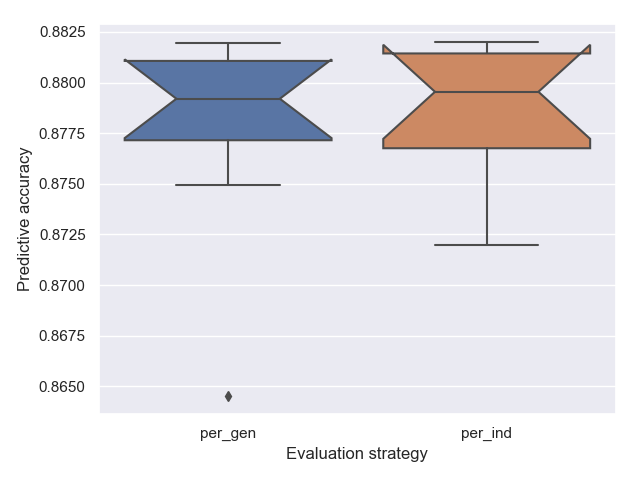
\includegraphics[width=0.9\textwidth]{../img/magic-out.png}
\caption{Comparison of strategies on the magic dataset}
\label{pic04:magic}
\end{figure}

\begin{figure}[ht]\centering
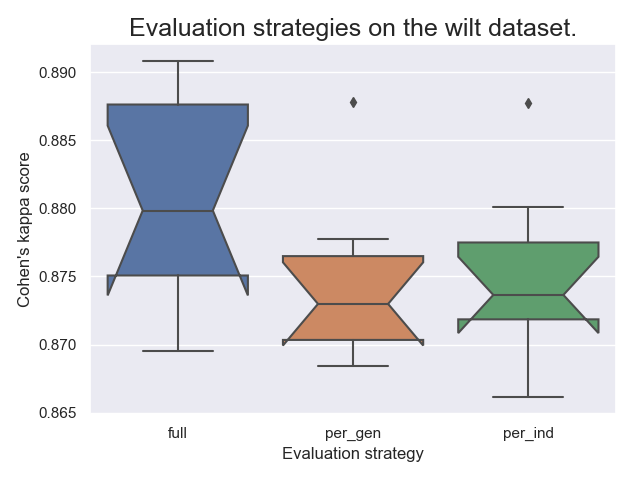
\includegraphics[width=0.9\textwidth]{../img/wilt-out.png}
\caption{Comparison of strategies on the wilt dataset}
\label{pic04:wilt}
\end{figure}

\begin{figure}[ht]\centering
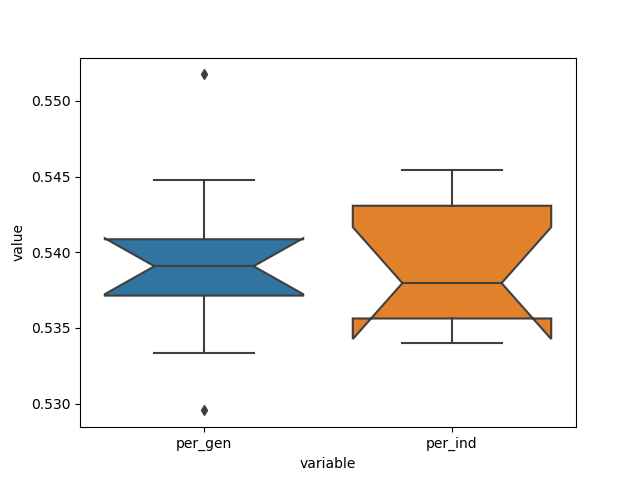
\includegraphics[width=0.9\textwidth]{../img/winequality-out.png}
\caption{Comparison of strategies on the wine-quality-white dataset}
\label{pic04:winequality}
\end{figure}

% goal - test relationship between per gen and per ind

% Take maximum

% test comparison + describe

% boxplots for comparison (seaborn)
%   - winequality
%   - wilt
%   - magic

% scipt that gets the maximums and makes the plot(s)


\section{Combinations of genetic operators} \label{sec:exp:genop}


\section{OpenML-CC18 benchmarking suite}
% OpenML-CC18
% benchmark description
The OpenML-CC18 suite is a set of classification tasks created for the purpose
of practical benchmarking. It contains 72 datasets available at OpenML
(\citep{openmlcc18}), where
every dataset is associated with one task --- a 10-fold cross-validation. The
datasets included in the suite have been frequently used in recently published
benchmarks and also satisfy several criteria, like a limit on instance count.
The full list of criteria can be found in the OpenML documentation
\cite{openmlcc18docs}.

\begin{sidewaysfigure}[ht]
    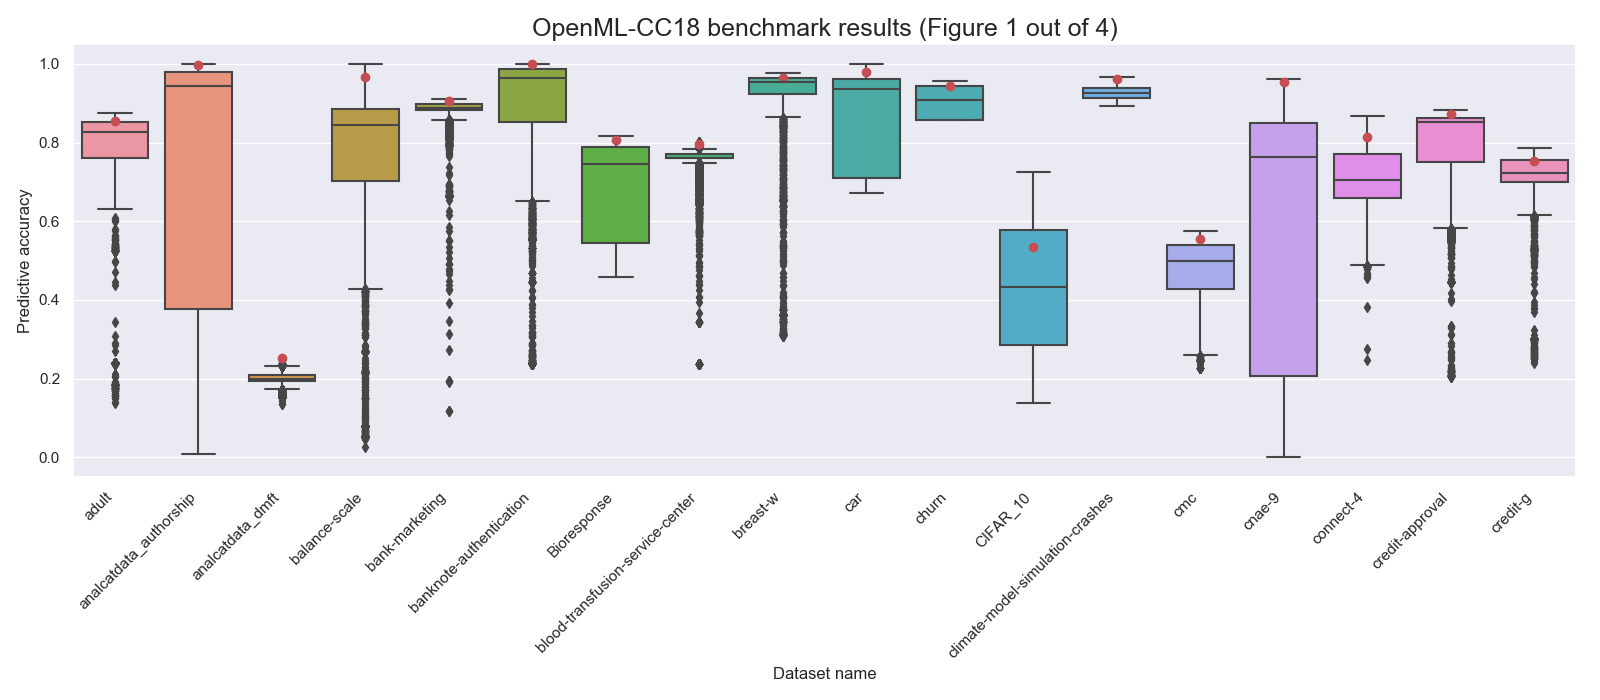
\includegraphics[width=\textwidth]{../img/openml-boxplot0.png}
    \caption[OpenML-CC18 benchmark result comparison (Figure 1 out of 4)]{
    OpenML-CC18 benchmark result comparison (Figure 1 out of 4).
    Boxplots visualize distributions of predictive accuracies of all
    runs uploaded to OpenML.}
    \label{fig:OpenML:boxplot:0}
\end{sidewaysfigure}

\begin{sidewaysfigure}[ht]
    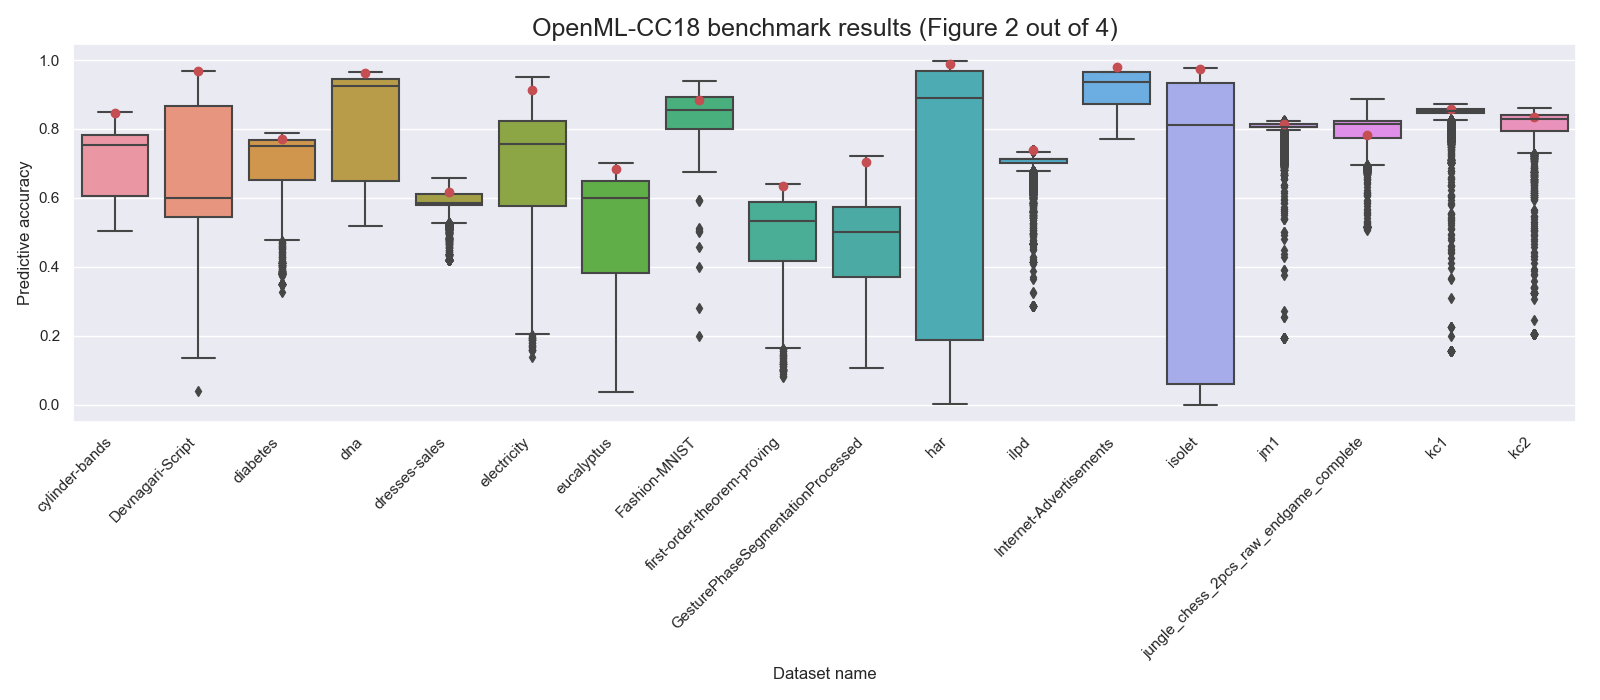
\includegraphics[width=\textwidth]{../img/openml-boxplot1.png}
    \caption[OpenML-CC18 benchmark result comparison (Figure 2 out of 4)]{
	OpenML-CC18 benchmark result comparison (Figure 2 out of 4).    
    Boxplots visualize distributions of predictive accuracies of all
    runs uploaded to OpenML.}
    \label{fig:OpenML:boxplot:1}
\end{sidewaysfigure}

\begin{sidewaysfigure}[ht]
    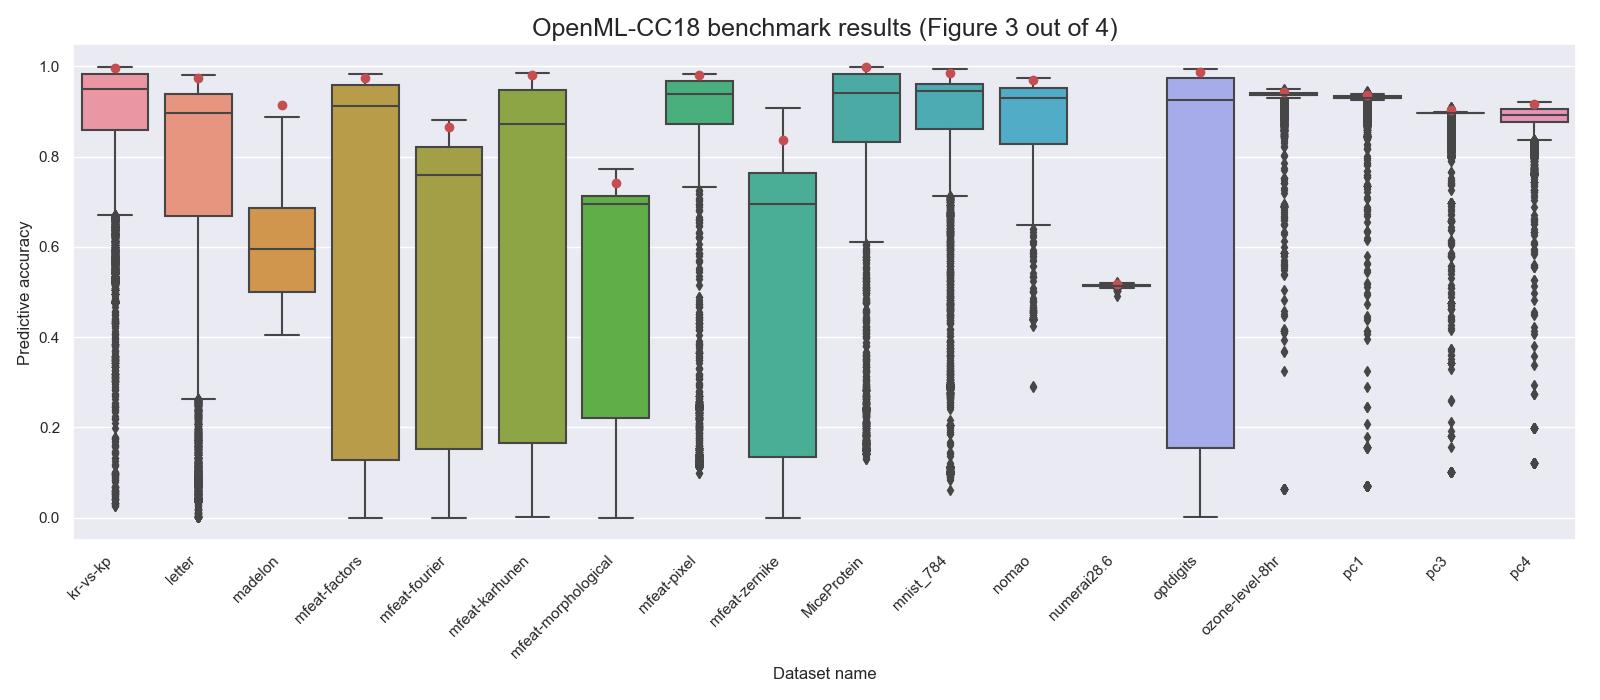
\includegraphics[width=\textwidth]{../img/openml-boxplot2.png}
    \caption[OpenML-CC18 benchmark result comparison (Figure 3 out of 4)]{
	OpenML-CC18 benchmark result comparison (Figure 3 out of 4).    
    Boxplots visualize distributions of predictive accuracies of all
    runs uploaded to OpenML.}
    \label{fig:OpenML:boxplot:2}
\end{sidewaysfigure}

\begin{sidewaysfigure}[ht]
    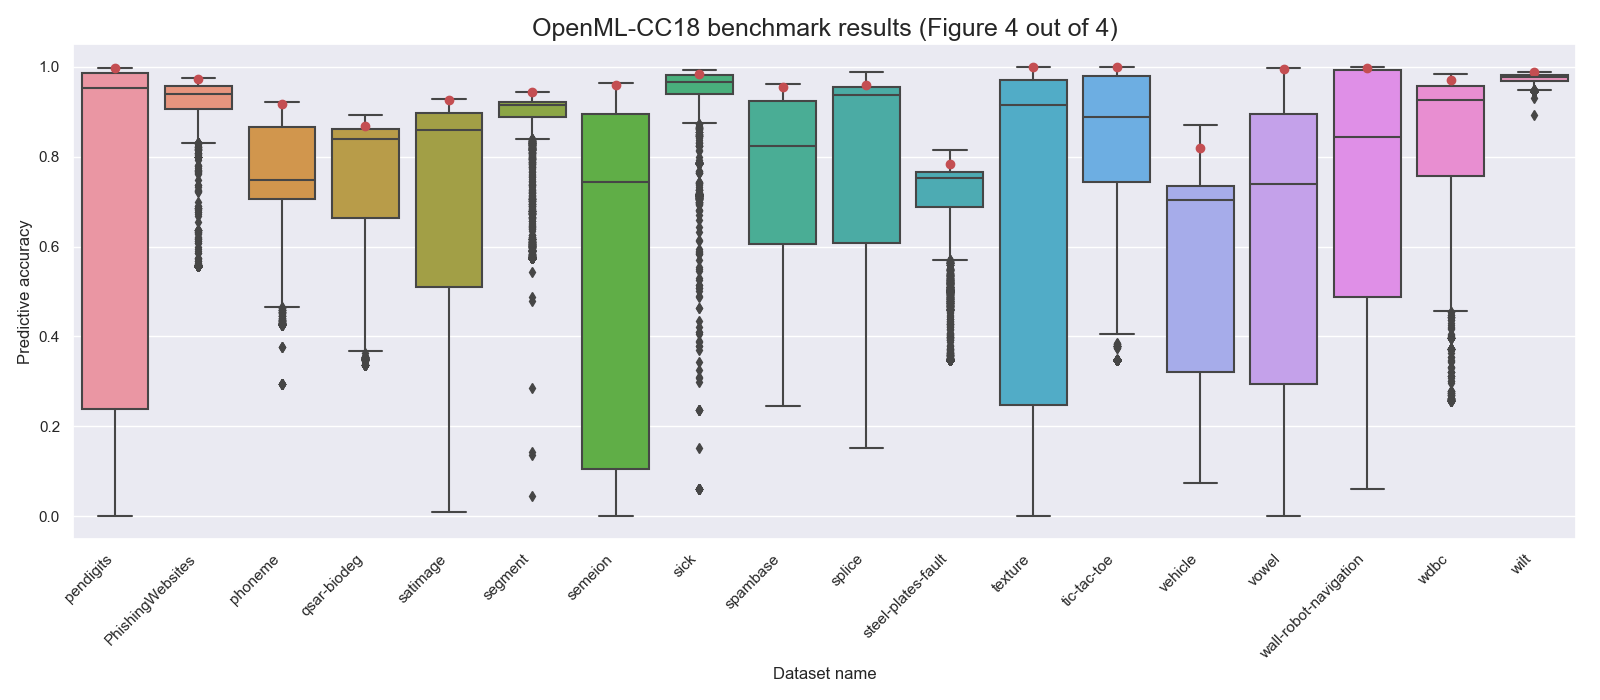
\includegraphics[width=\textwidth]{../img/openml-boxplot3.png}
    \caption[OpenML-CC18 benchmark result comparison (Figure 4 out of 4)]{
    OpenML-CC18 benchmark result comparison (Figure 4 out of 4).
    Boxplots visualize distributions of predictive accuracies of all
    runs uploaded to OpenML.}
    \label{fig:OpenML:boxplot:3}
\end{sidewaysfigure}